\documentclass[a4paper,11pt]{article}
\usepackage{a4wide}
\usepackage{graphicx}
\usepackage{url}
\usepackage[utf8]{inputenc}
\usepackage[T1]{fontenc}
\usepackage[czech]{babel}

% vim: spl=cs:


%postup při řešení, způsob řešení
%dosažené cíle
%zdůvodnění případných změn v řešení projektu (technické změny, nikoliv finanční)
%konkrétní výstupy, další využitelnost
%přínosy projektu, vlastní hodnocení
%tisková zpráva – 2 řádky textu (cca 300 znaků) s odkazem na web řešitele

\title{Analýza dat z hmotnostní spektrometrie \\ za použití strojového učení \\[\medskipamount] 
\normalsize
závěrečná zpráva projektu FR CESNET}
\author{Aleš Křenek, Michal Starý, Adam Hájek, (Jiří Novotný)}
\date{\today}

\begin{document}
\maketitle

%\section{Anotace}
\begin{abstract}

Cílem projektu je přenesení prototypů software pro zpracování dat z hmotností
spektrometrie metodami strojového učení na výpočetní zdroje e-INFRA CZ a
vyhodnocení chování těchto algoritmů na dostupných architekturách akcelerátorů
GPU. Práce se zaměří na řešení problémů spojených s velkými objemy dat, jako
třeba distribuované výpočty nebo současné využití více akcelerátorů, a které
bez použití zdrojů e-INFRA nebylo možné řešit. Projekt navazuje na širší
činnost společné výzkumné skupiny centra Recetox a Ústavu výpočetní techniky MU,
která se zabývá mimo jiné i vývojem těchto metod. Přínosem pro aplikační oblast
bude posun ve vývoji prototypů k aplikovatelnosti na rozsáhlé a pro
kompetitivní výzkum nezbytné datové sady. Přínosem pro e-INFRA CZ bude zejména
zkušenost s přenesením a provozem této třídy aplikací na infrastruktuře a
případná zpětná vazba potřebná k jejímu dalšímu rozvoji, jako například
vhodnost konkrétního HW či změny SW prostředí.

\end{abstract}

\section{Postup a způsob řešení}

\subsection{Hmotnostní spektrometrie a strojové učení}

Hmotnostní spektrometrie je experimentální technika, jejíž hlavním cílem je v~základním 
režimu použití potvrzení či vyvrácení přítomnosti konkrétních sloučenin ve zkoumaném vzorku.
Takto je např.\ používána při bezpečnostních kontrolách, kde se zaměřuje na detekci stop manipulace s~výbušninami.

Pro vědecké aplikace je ale významnější a větší výzvu představuje tzv.\ \emph{necílený} (untargeted) režim.
Cílem je zde zjistit pokud možno kompletní složení vzorku přes danou třídu sloučenin (např.\ molekuly daného rozsahu velikosti/hmotnosti).
Použití této techniky je velmi široké, vzorky mohou pocházet z~životního prostředí (půda, voda, i vzduch),
rostlin, potravin, i od lidí (typicky se zkoumají produkty metabolismu, tj.\ vzorky krve, moči a stolice).

\begin{figure}
\begin{center}
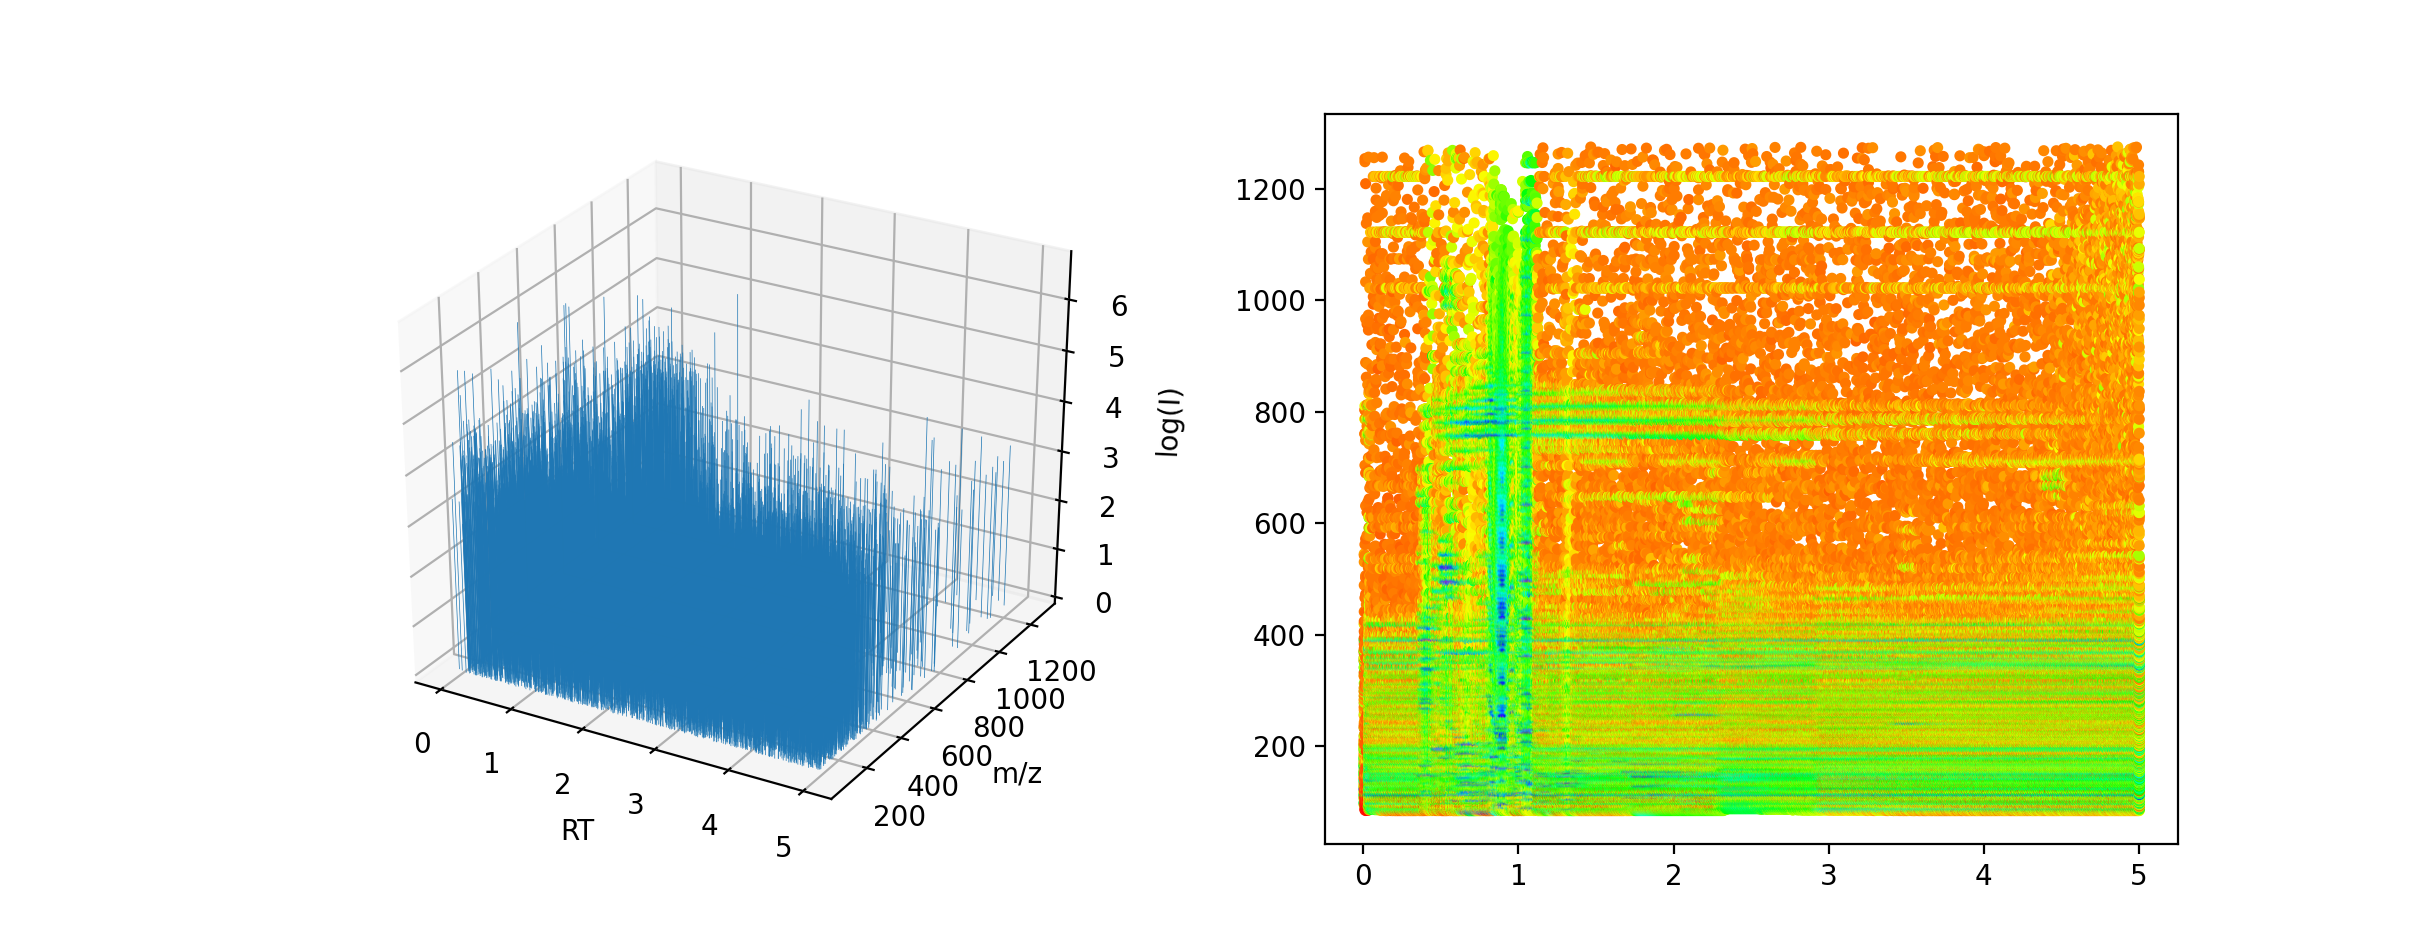
\includegraphics[width=.8\hsize]{sample}
\end{center}
\caption{Ukázka vzorku dat naměřených hmotnostní spektrometrií. Vlevo
třírozměrné zobrazení intenzity signálu pro konkrétní kombinace retenčního času
(\emph{RT}) a hmotnosti ($m/z$), vpravo tatáž data s~barevným kódováním intenzity}
 \label{f:ms}
\end{figure}


Po laboratorním zpracování vzorku (oddělení zajímavé třídy sloučenin, vyčištění, úprava koncentrace \dots)
je typickým dalším krokem kapalinová nebo plynná chromatografie, která od sebe oddělí jednotlivé sloučeniny
ve vzorku, ty se v~konkrétním \emph{retenčním čase} (\emph{RT}) následně dostávají do samotného hmotnostního spektrometru.
Tam jsou nejprve ionizovány, a to buď tzv.\ \emph{měkce},
kdy molekuly pouze získávají náboj a jsou minimálně fragmentovány,
nebo \emph{tvrdě}, kdy je většina molekul ,,rozbita`` na menší elektricky nabité fragmenty.
Pro naše účely (ve spolupráci s~centrem Recetox) se zaměřujeme na druhou variantu.
Hmotnostní spektrometry pak různými způsoby detekují dráhu pohybujících se nabitých částic v~elektrickém poli;
na základě jejich analýzy pak lze určit poměr hmotnosti a náboje ($m/z$) jednotlivých částic.
Jejich souhrn pak tvoří hmotnostní spektrum, které je charakteristické pro konkrétní původní sloučeninu,
a tu tedy lze na jeho základě identifikovat.
Obrázek~\ref{f:ms} ukazuje typická naměřená data.

Data jsou následně výpočetně zpracována (konvenčními metodami), dochází k~odfiltrování šumu, dekonvoluci signálu v~čase,
a korekci artefaktů měření na konkrétním přístroji.
Postupů k~těmto účelům bylo vyvinuto mnoho, a nejsou předmětem tohoto projektu.
Výsledkem pak je posloupnost jednotlivých \emph{hmotnostních spekter}, viz např.\ obr.~\ref{f:thc},
která už patří jednotlivým odděleným sloučeninám.
Konvenční metody pak tato spektra vyhledávají na základě podobnosti v~databázích známých sloučenin,
a~tak jsou sloučeniny identifikovány.

\begin{figure}
\begin{center}
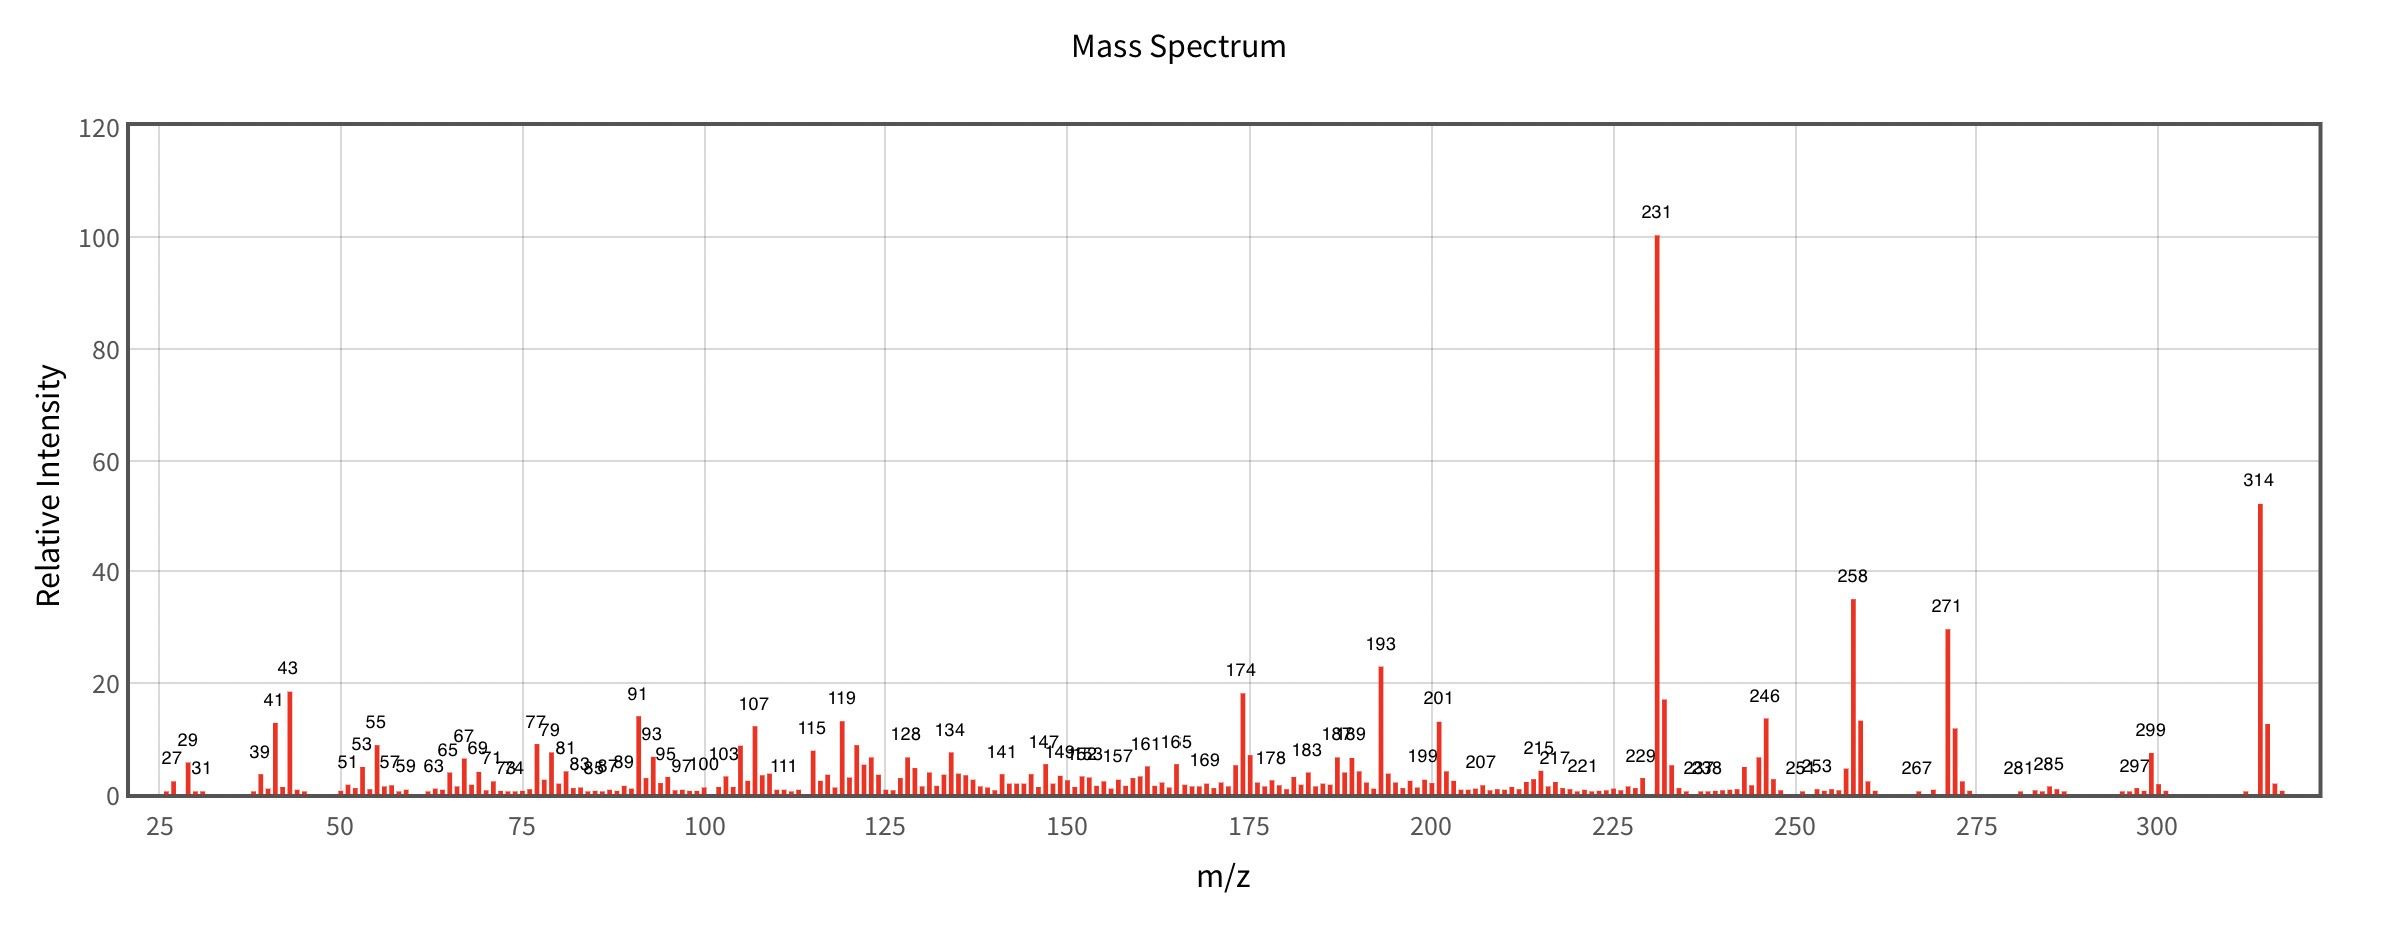
\includegraphics[width=.8\hsize]{thc}
\end{center}
\caption{Ukázka extrahovaného hmotnostního spektra jedné sloučeniny (tetrahydrocannabinol)}
\label{f:thc}
\end{figure}

Výpočetní metody, které realizují výše naznačený postup, jsou komplikované, trpí mnohými nedostatky,
a rozvíjejí se už dekády.
Je tedy zcela přirozené, že v~posledních letech bylo učiněno mnoho pokusů, jak některé nedostatky 
konvenčních metod překonat technikami strojového učení (i jejich stručný výčet by překonal rozsah této zprávy).
V~tomto projektu se zaměřujeme na dvě oblasti, které byly identifikovány ve spolupráci s~centrem Recetox jako potřebné.
Jim jsou věnovány následující části textu.

Pro trénování a vyhodnocení modelů byla použita databáze NIST~\cite{nist}, po předzpracování obsahující
cca.~290~tis.\ záznamů. 
Tato sada byla dále rozdělena na trénovací, validační a testovací,
s~ohledem na skutečnost, že záznamy v~ní nejsou unikátní (v~řadě případů existuje více spekter k~jedné sloučenině) --
zajišťujeme, že sloučeniny reprezentované i různými spektry, se nevyskytují v~trénovací, validační a testovací sadě
současně. 

\subsection{Doplnění chybějícího signálu ve spektrech sloučenin\\ s~nízkou koncentrací}

Zpracování signálu hmotnostní spektrometrie ve fázích odstranění šumu a dekonvoluce je vždy předmětem kompromisu.
Příliš tolerantní nastavení těchto postupů způsobí, že šum, případně přesahy chromatografie v~širším časovém okně jsou
považovány za signál skutečných sloučenin, výsledná spektra jsou příliš ,,zahuštěná`` a následující kroky identifikace
sloučenin jsou pak nepřípustně zatíženy falešnými pozitivy.
Proto je zpravidla nezbytné striktnější nastavení prahů detekce šumu, rozsahu chromatografických špiček a dalších parametrů
zpracování.
V~případě výskytu sloučenin v~nízké koncentraci, což je ale pro mnoho aplikací právě to zajímavé (např.\ běžné metabolity
v~krevní plazmě jsou očekávány i ve vysoké koncentraci, ale hledáme stopy projevů znečištění životního prostředí
pesticidy), metody identifikují slabý signál jako šum, do výsledných spekter se nepromítne, a identifikace je pak zatížena
falešnými negativy.

Řešením tohoto problému se v~projektu zabýval zejména Michal Starý a výsledky jsou i předmětem jeho bakalářské práce.
Identifikovali jsme dva odlišné scénáře -- falešná negativa zanesená příliš agresivní detekcí šumu, kdy jsou ze spekter
chybně odstraněny špičky slabého signálu, a chybějící špičky v~důsledku nedokonalé dekonvoluce, kdy je zpravidla
i relativně silný signál přiřazen do špatného časového okna (tento problém je symetrický, jeho druhou stranou, kdy se 
ve spektru objeví část signálu patřící do jiného času, jsme se prozatím nezabývali, protože pro identifikaci sloučenin
není tak kritický).


% metody
Prvním krokem potřebným pro aplikaci technik strojového učení je vhodná reprezentace 
vstupních dat, tzv.~\emph{embedding}. Použili jsme metodu odvozenou z~publikované metody Spec2Vec~\cite{spec2vec},
která vychází z~technik používaných při zpracování přirozeného jazyka.
Metoda je trénována na reálných datech tak, aby každé špičce přiřadila vektor v~300 rozměrném prostoru tak,
že špičky vyskytující se ve spektrech společně jsou zobrazeny na vzájemně blízké vektory.
Reprezentací celého spektra je pak součet vektorů jednotlivých špiček vážený jejich intenzitou.
Detaily viz příloha~C práce~\cite{stary}.

Pro samotnou predikci chybějících špiček 
uvažujeme danou konstantu $k$ -- počet spolehlivě detekovaných špiček nejvyšší intenzity,
které jsou vstupem predikčního modelu, a jeho úkolem je doplnit (i opakovaně) další. 
Byly vyhodnoceny následující modely:
\begin{itemize}
\item \emph{kNN.} Trénovací sada je zde použita jako databáze, v~níž je vyhledáno $nk$ nejbližších 
záznamů ke vstupu (kde $n$ je hyperparametrem modelu s~použitými hodnotami 1,3,5,10). 
Takto získaná spektra jsou zprůměrována a po vyloučení překryvů se vstupem jsou výstupem špičky setříděné
podle celkové intenzity.
Dalším hyperparametrem metody je metrika použitá k~vyhledávání podobností, používáme cosinovou podobnost
a vzdálenost embeddingu (viz předchozí odstavec).
Tato metoda je jednoduchá a relativně naivní, byla použita zejména pro stanovení startovací čáry pro hodnocení
dalších metod.
\item \emph{MLP} (\emph{Multi-Layer Perceptron}) je nejjednodušším modelem
neuronové sítě, experimentovali jsem s~modely o jedné až třech vrstvách o
velikosti 500 a 1000 neuronů.
\item \emph{LSTM} je založena na architektuře tzv.~\emph{Long-Short Term Memory} rekurentní neuronové sítě.
Vyzkoušeli jsme tři varianty modelu -- s~náhodnou inicializací embeddingu, jeho předtrénováním, a se zafixovaným embddingem.
Všechny byly aplikovány autoregresivně (výstup jedné iterace je vstupem následující) a přímo, s~extrakcí špiček z~predikované distribuce.
% v Bc 2 hodiny @ A100

\item \emph{GPT-2.} Je postavena na architektuře takto označené architektuře neuronové sítě
která využívá koncept transformeru.
Nicméně i ,,malá`` varianta používaná pro jazykové modely obsahuje 80 mil.\ trénovaných parametrů,
což je pro naše účely neadekvátně mnoho. Proto používáme redukované varianty s~10, resp. 40 mil.\ parametrů.
Pro špičky (resp. jejich hodnoty $m/z$) je použitý výše popsaný embedding, celé spektrum je zakódováno do vektoru
o 300 složkách.
Podobně jako v~jazykových modelech, kde je dalším vstupním kanálem pořadí slova ve větě,
tímto způsobem do modelu vstupuje intenzita špiček, experimentovali jsme s~jejím kvantováním do 256 úrovní
na lineární a kvadratické škále.
% 10 h @ A100


\end{itemize}

\begin{figure}
\begin{center}
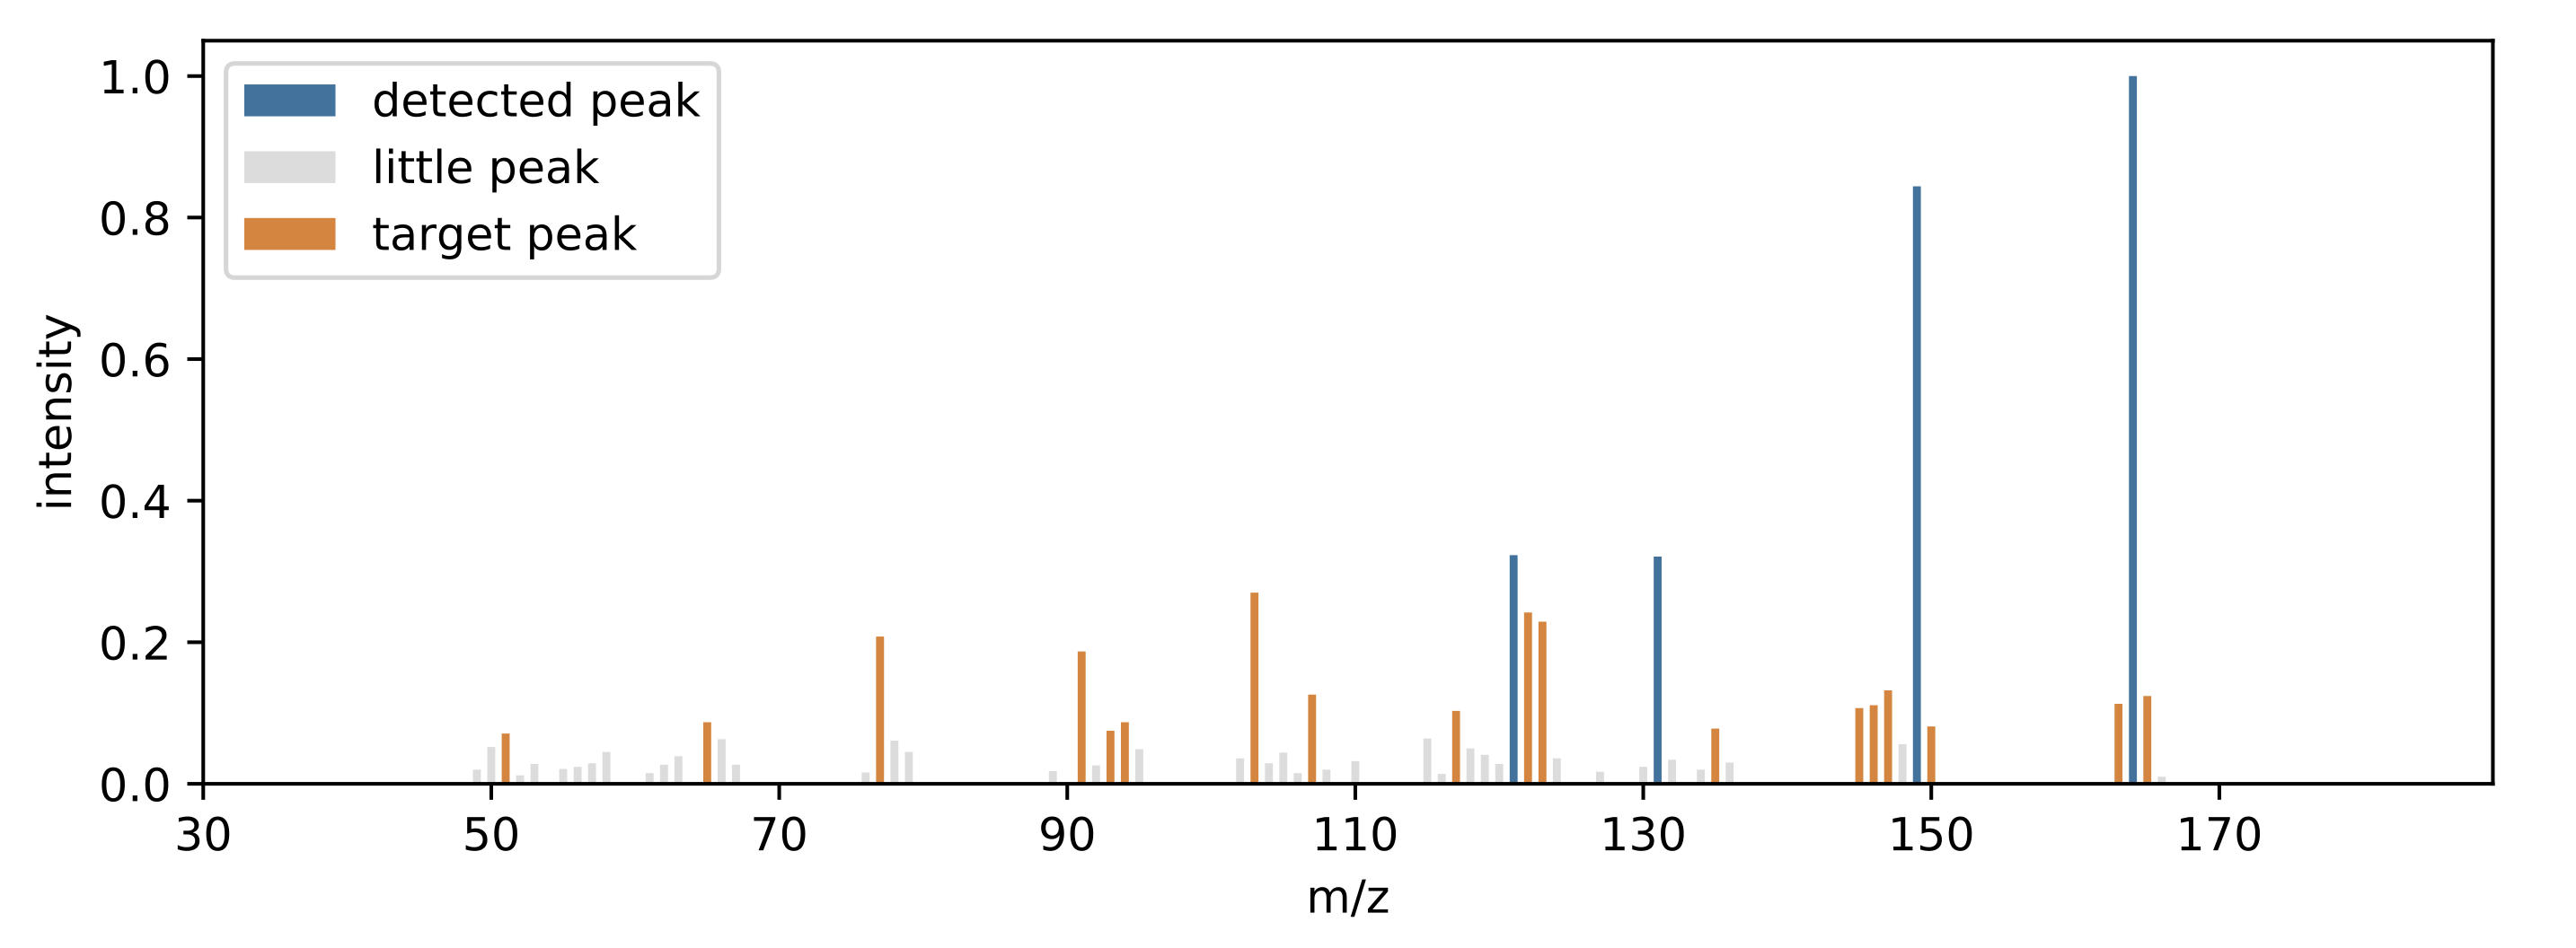
\includegraphics[width=.8\hsize]{metric-missing}
\end{center}
\caption{Konstrukce metriky doplnění chybějících špiček na konkrétním příkladu, první scénář.
Modře jsou označeny vstupní špičky pro model ($k=4$), oranžově očekávané výsledky.
Pokud např. model detekuje správně špičky na hodnotách $m/z$ 77, 91, 151, 135 (a dalších 14 detekovaných se
s~očekávanými neshoduje), byla přesnost modelu $4/18 = 0.22$
}
\label{f:metric-missing}
\end{figure}

Pro vyhodnocení úspěšnosti a relativní porovnání metod je třeba definovat exaktní metriky.
Pro první scénář (příliš agresivní odstranění šumu) ji 
neformálně ilustruje obrázek~\ref{f:metric-missing}.
Podle dané konstanty~$k$ uvažujeme počet detekovaných špiček, které jsou vstupem pro metodu,
a prahovou hodnotu (empiricky určenou jako 20~\%) relativní intenzity proti $k$-té špičce,
která je ještě považována za významnou. 
U každého testovacího spektra pak identifikujeme množinu špiček, které jsou menší než prvních~$k$,
ale jejichž intenzita je nad prahovou hodnotou, a testovaný model necháme doplnit stejný počet špiček.
Za metriku volíme \emph{přesnost} (precision) této predikce, tj.\ podíl počtu správně identifikovaných špiček
a~celkového počtu očekávaných/doplněných.
Formálně je metrika definována v~příloze~B práce~\cite{stary}. 

Pro druhý scénář (chyby dekonvoluce) používáme mírně odlišnou metriku (obr.~\ref{f:metric-wrong}).
Protože se v~tomto případě může model dopouštět dvou druhů chyb -- falešná negativa (FN), tj.\ nedetekuje špičky tam,
kde by měly být, a falešná pozitiva (FP), detekované špičky na místech, kde být nemají,
výslednou metriku počítáme jako skóre F1.

\begin{figure}
\begin{center}
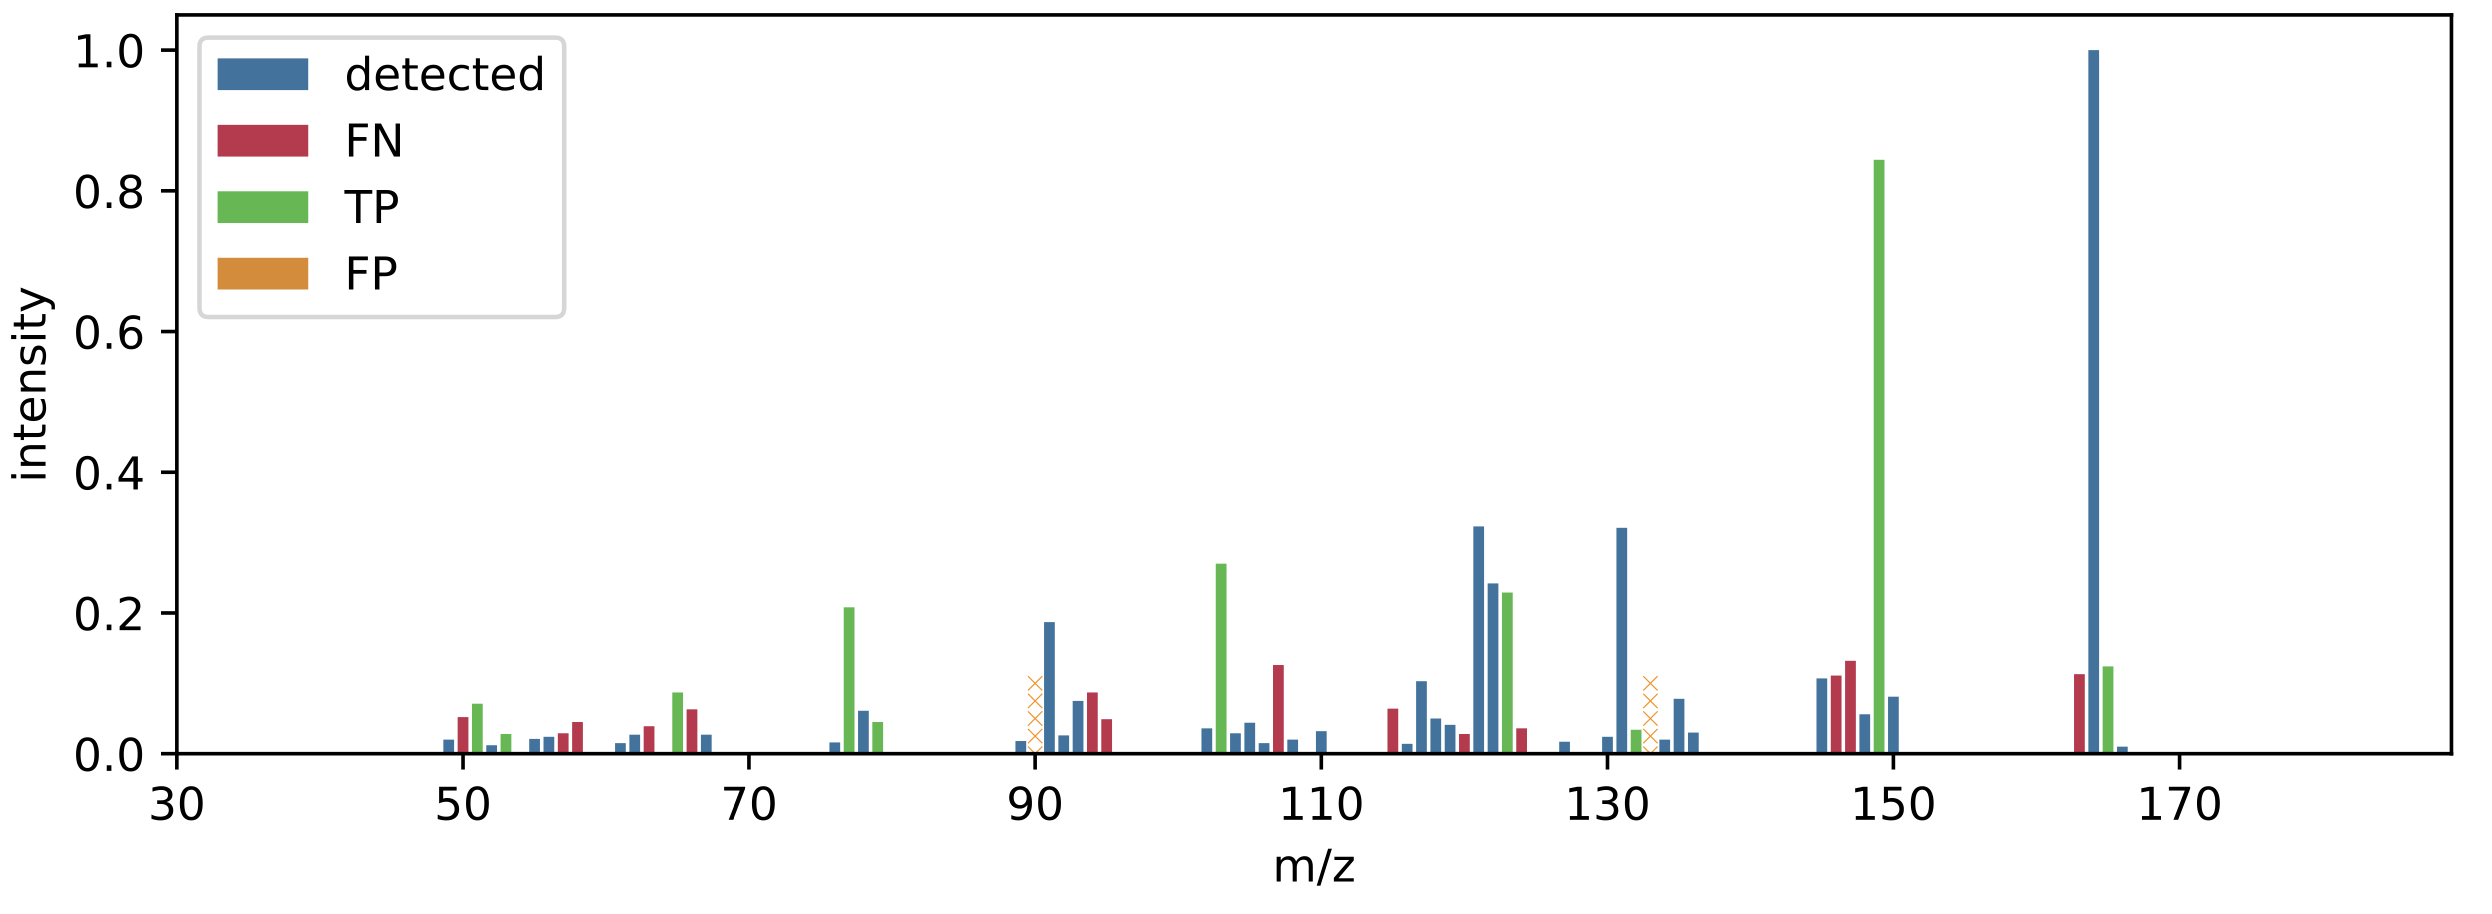
\includegraphics[width=.8\hsize]{metric-wrong}
\end{center}
\caption{Konstrukce metriky doplnění chybějících špiček na konkrétním příkladu, druhý scénář.
Vstupem pro model jsou modře vyznačené špičky. Model detekoval korektně špičky zelené (TP),
nepodařilo se mu detekovat očekávané červené špičky (FN), ale predikoval špičky špatně na
místech označených žlutými křížky (FP).
}
\label{f:metric-wrong}
\end{figure}

Výsledky jsou detailněji diskutovány v~části~\ref{cile}.

Pro vývoj a testování kódu jsme používali zejména databázi hmotnostních spekter
NIST~\cite{nist} ve verzi z~roku 2021.
Tato databáze nám byla poskytnuta spolupracujícím centrem Recetox, není však veřejně dostupná.
Proto pro účely benchmarku popisovaných dále v~této zprávě používáme menší, ale stále dostatečně reprezentativní
veřejně dostupnou databázi MoNA~\cite{mona}.

Implementace modelů strojového učení využívá nízkoúrovňový framework \emph{PyTorch}, který poskytuje
potřebné nástroje pro sestavení, trénování a použití neuronových sítí a dovoluje výpočty transparentně
přesměrovat na akcelerátory (v~našem případě GPU).
Dále využíváme vysokoúrovňovou knihovnu \emph{PytorchLightning}, která dovoluje řadu kroků
je implementuje řadu opakovaných kroků standardizovaným způsobem a dovoluje tak vývoj konkrétních aplikací
značně zjednodušit a automatizovat.
Výše popsaný model GPT-2 je postaven na implementaci \emph{HuggingFace transformers.}
Pro zaznamenání a analýzu průběhu výpočtu používáme knihovnu \emph{Weights \& Biases} včetně vizualizace na webové aplikaci
\url{https://wandb.ai/}.
Prímární uživatelské rozhraní pro trénování a použití modelů a benchmarky je implementováno v~prostředí
\emph{Jupyter Notebook}.
Komplexní softwarové prostředí zahrnující všechny výše uvedené komponenty je zapouzdřeno do
obrazů kontejneru \emph{Docker}.
Kontejnery je následně možno spouštět v~principu kdykoli, od uživatelské pracovní stanice přes
infrastrukturní službu \emph{Kubernetes} i na běžných výpočetních uzlech Metacentra s~využitím 
prostředí \emph{Singularity.} 

V~posledním jmenovaném byly provedeny i systematické experimenty pro vyhodnocení výkonu (benchmark).
Pro tyto účely vybíráme model GPT-2, který je vhodně flexibilní v~hyperparametrech ovlivňujících jeho velikost,
přitom při použití na vstupní databázi MoNA výpočet probíhá realisticky a v~časovém rozpětí vhodném
pro účely benchmarku (nižší desítky minut).
Tytéž výpočty na obsáhlejší datové sadě NIST a stejném hardware trvají hodiny až dny, což je pro účely
již nadbytečné a nepraktické.

Základem benchmarku je vzor shellového skriptu, do nějž uživatel vloží požadované množiny hodnot proměnlivých parametrů: 
\begin{itemize}
\item počty hlav transformeru a jejich vrstev (bloků) a šířka embeddingu -- hyperparametry zásadně ovlivňující velikost modelu GPT-2;
\item velikost dávky -- jeden z~nejběžnějších hyperparametrů, kromě dopadu na konvergenci také určuje náročnost výpočtu na 
paměť;
\item numerická přesnost, možné volby jsou 32 (jednoduchá) a 16 (poloviční,
resp.\ smíšená) bitů -- nejnovější generace akcelerátorů dosahují ve smíšené přesnosti
vyššího výkonu bez výrazného dopadu na celkovou přesnost;
\item počet použitých GPU;
\item cluster Metacentra (vlastnost uzlů v~dávkovém systému PBS), na kterém bude výpočet spuštěn.
\end{itemize} 
Skript vygeneruje pro každou kombinaci hodnot těchto parametrů zadání úlohy ke spuštění v~Metacentru,
heuristickým výpočtem odhadne horní limit nároků na zdroje (zejména paměť a počet jader CPU), a úlohy
zadá do dávkového systému PBS.
Dále je pro zadání těchto úloh vyžadováno jméno projektu a autentizační klíč pro službu Weights \& Biases.
Úlohy do ní za běhu zaznamenávají charakteristiky průběhu výpočtů, které tak lze sledovat a analyzovat
již za běhu na webovém rozhraní služby.
Jednotlivé úlohy jsou automaticky označny (tzv.~\emph{tags} ve W\&B) konkrétními hodnotami parametrů
(hlavy, vrstvy, dávka, \dots) tak, aby bylo možno v~systému snadno vybírat jejich podmnožiny
pro další analýzu.

\subsection{Identifikace neznámých sloučenin}
Potenciálně problematickým místem zpracování dat z~hmotnostní spektrometrie je identifikace sloučenin,
kterou konvenční metody realizují podobnostním hledáním ve spektrálních databázích.
Zmíněná databáze NIST obsahuje cca.\ 300~tis. spekter, žádné další databáze nejsou obsáhlejší.
Přitom popsána byla popsána téměř miliarda sloučenin relevantní velikosti (databáze ZINC~\cite{zinc}),
odhady říkají, že v~přírodě se může vyskytovat až $10^{60}$ takových sloučenin.
Pravděpodobnost, že pro náhodně získané spektrum najdeme odpovídající záznam v~databázi, je tedy velmi nízká.

Tento problém se snaží řešit tzv.\ \emph{de-novo} identifikační metody.
V~poslední době byly publikovány čtyři na sobě nezávislé~\cite{msnovelist, massgenie, vaems, spec2mol},
které shodně využívají obdobného postupu.
Vstupem je databáze existujících (nebo alespoň pravděpodobných) molekul jako ZINC.
Pro tuto databázi jsou různými postupy vygenerována předpokládaná spektra (mohou být použity ,,expertní`` modely,
které nějakým způsobem zachycují mechanismus vzniku nabitých fragmentů, i pomocné modely strojového učení
natrénované na existujících malých databázích spekter); 
tato spektra jsou relativně nepřesná, ale výhodou je, že takto lze získat jejich řádově větší počet.
Vygenerovaná spektra tvoří už dostatečně velkou trénovací sady pro modely strojového učení inspirované
zpracováním přirozeného jazyka -- problém je tak převeden na překlad z ,,jazyka spekter`` do ,,jazyka chemických vzorců``.

V projektu jsme se nejprve zabývali aplikací nejvyzrálejšího z~publikovaných modelů, MSNovelist~\cite{msnovelist}
na typ dat, která získáváme v~centru Recetox.
Narazili jsme ale na principiální omezení -- MSNovelist vyžaduje jako podstatný vstup tzv.~\emph{precursor ion},
známou hmotnost celé sloučeniny; ta je měřitelná v~experimentech LC/MS$^2$, pro něž byl MSNovelist vyvinut,
ale není dostupná v~našem experimentálním uspořádání GC/MS.

Proto jsme se začali věnovat dalšímu modelu MassGenie~\cite{massgenie}, pro nějž ale existuje pouze
zevrubný popis metody, zdrojové kódy nebyly publikovány.
V~době řešení projektu se podařilo navrhnout celý postup,
jeho schéma je na obr.~\ref{f:denovo}.
Použili jsme natrénovaný pomocný model NEIMS~\cite{neims} (architektura MLP),
syntetická spektra jím generujeme z~vybrané podmnožiny databáze ZINC (celkem 4.6 milionu spekter,
tj.\ stále ještě relativně malá část).
Na těchto spektrech trénujeme model transformeru (BART z~implementace HuggingFace).
Tuto část projektu měl na starosti především Adam Hájek.



\begin{figure}
\begin{center}
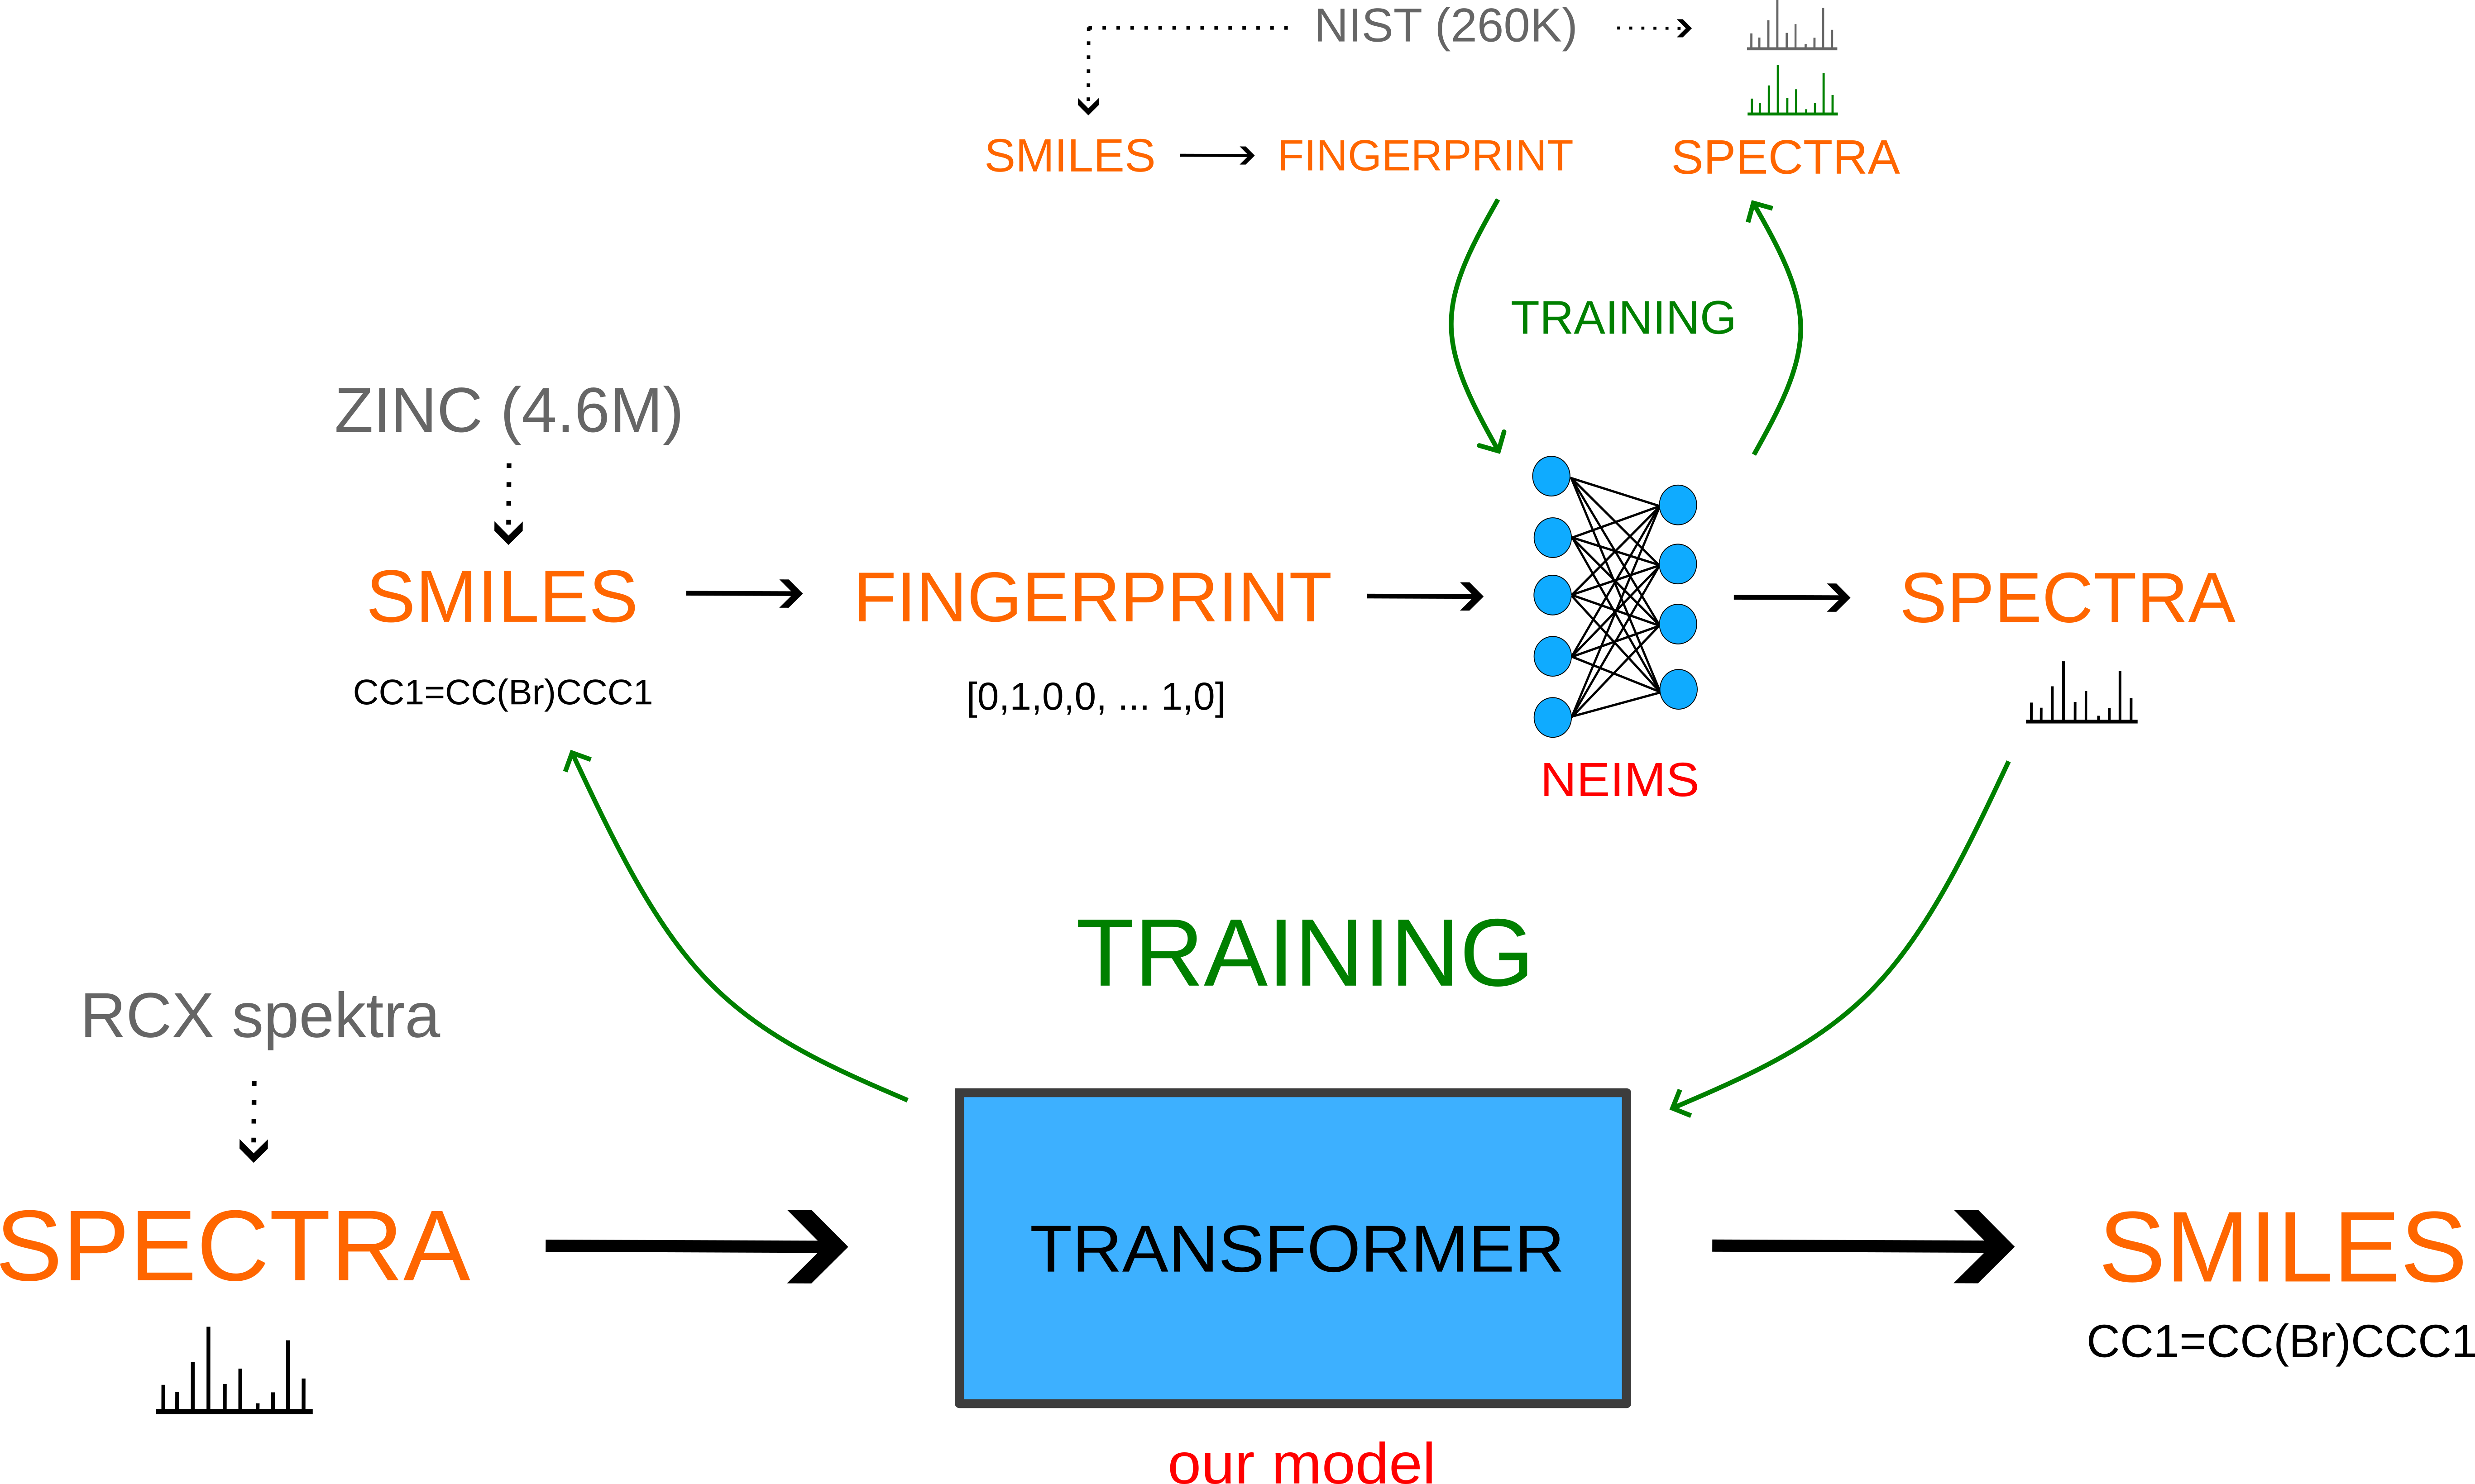
\includegraphics[width=.8\hsize]{diagram_whole}
\caption{Celkové schéma trénování de-novo modelu}
\label{f:denovo}
\end{center}
\end{figure}


% co je MS

% identifikované problémy v MS vhodné pro strojové učení, je jich hromada, nás zajímají tyhle dva

% implementace včetně tech detailů, frameworky, docker, wandb ...

% chybějící peaky ve spektru -- opsané z diplomky

% de-novo identifikace -- co má Adam


% benchmark




\section{Dosažené cíle, konkrétní výstupy a další využitelnost}
\label{cile}


% vyzkoušelo se několik metod doplnění peaků, fungují docela dobře
% jak to funguje, obrázky z bakalářky

V projektu jsme navrhli, implementovali, a důkladně otestovali (v~rozšířených variantách scénářů)
výše uvedené metody doplnění chybějích špiček ve spektrech.
Hlavní testování proběhlo na databázi NIST, kdy testovací sady byly generovány synteticky
odstraněním náhodně vybíraných špiček tak, aby bylo možno precizně vyhodnotit metriky 
úspěšnosti jednotlivých modelů.
Hlavní výsledky pro první scénář (agresivní odstranění šumu) ukazuje obr.~\ref{f:result-missing}.
Výrazně nejlépe se zde chová model GPT-2 (v~redukované variantě s~6 hlavami a vrstvami; větší modely neměly
žádný měřitelný přínos), dosahuje 60\% přesnosti.
Složitost modelu (která je zde řádově vyšší než u dalších variant) je zde opodstatněná,
model je přesvědčivě schopen postihnout charakteristiky dat lépe.
Ve druhém scénáři (chyby dekonvoluce) hlavní výsledky shrnuje obr.~\ref{f:result-wrong}.
Nejlepších výsledků zde opět dosahuje nejsložitější model (MLP), až do úrovně pravděpodobnosti chybějící špičky
(tj.\ relativního množství chybějících špiček včetně těch nejvýznamnějších) 40~\% je hodnota skóre~F1 nad úrovní
60~\%. To lze interpretovat tak, že model s~touto úspěšností chybějící špičky detekuje
a současně negeneruje ve větší míře falešná pozitiva.
Přestože se jedná o nejjednodušší možnou architekturu neuronové sítě, dostatečně velký model
je zde opět s~to zachytit podstatné rysy trénovací datové sady.
Scénáře testování a rozsáhlejší sady výsledku jsou uvedeny a
detailně diskutovány v~bakalářské práci Michala Starého~\cite{stary}.
Ta je na běžná měřítka bakalářské práce nadstandardně kvalitní a obsáhlá 
a byla oceněna cenou děkana FI MU za vynikající závěrečnou práci.
Součástí elektronické přílohy této práce je i kompletní implementace a návod k~použití.

\begin{figure}
\begin{center}
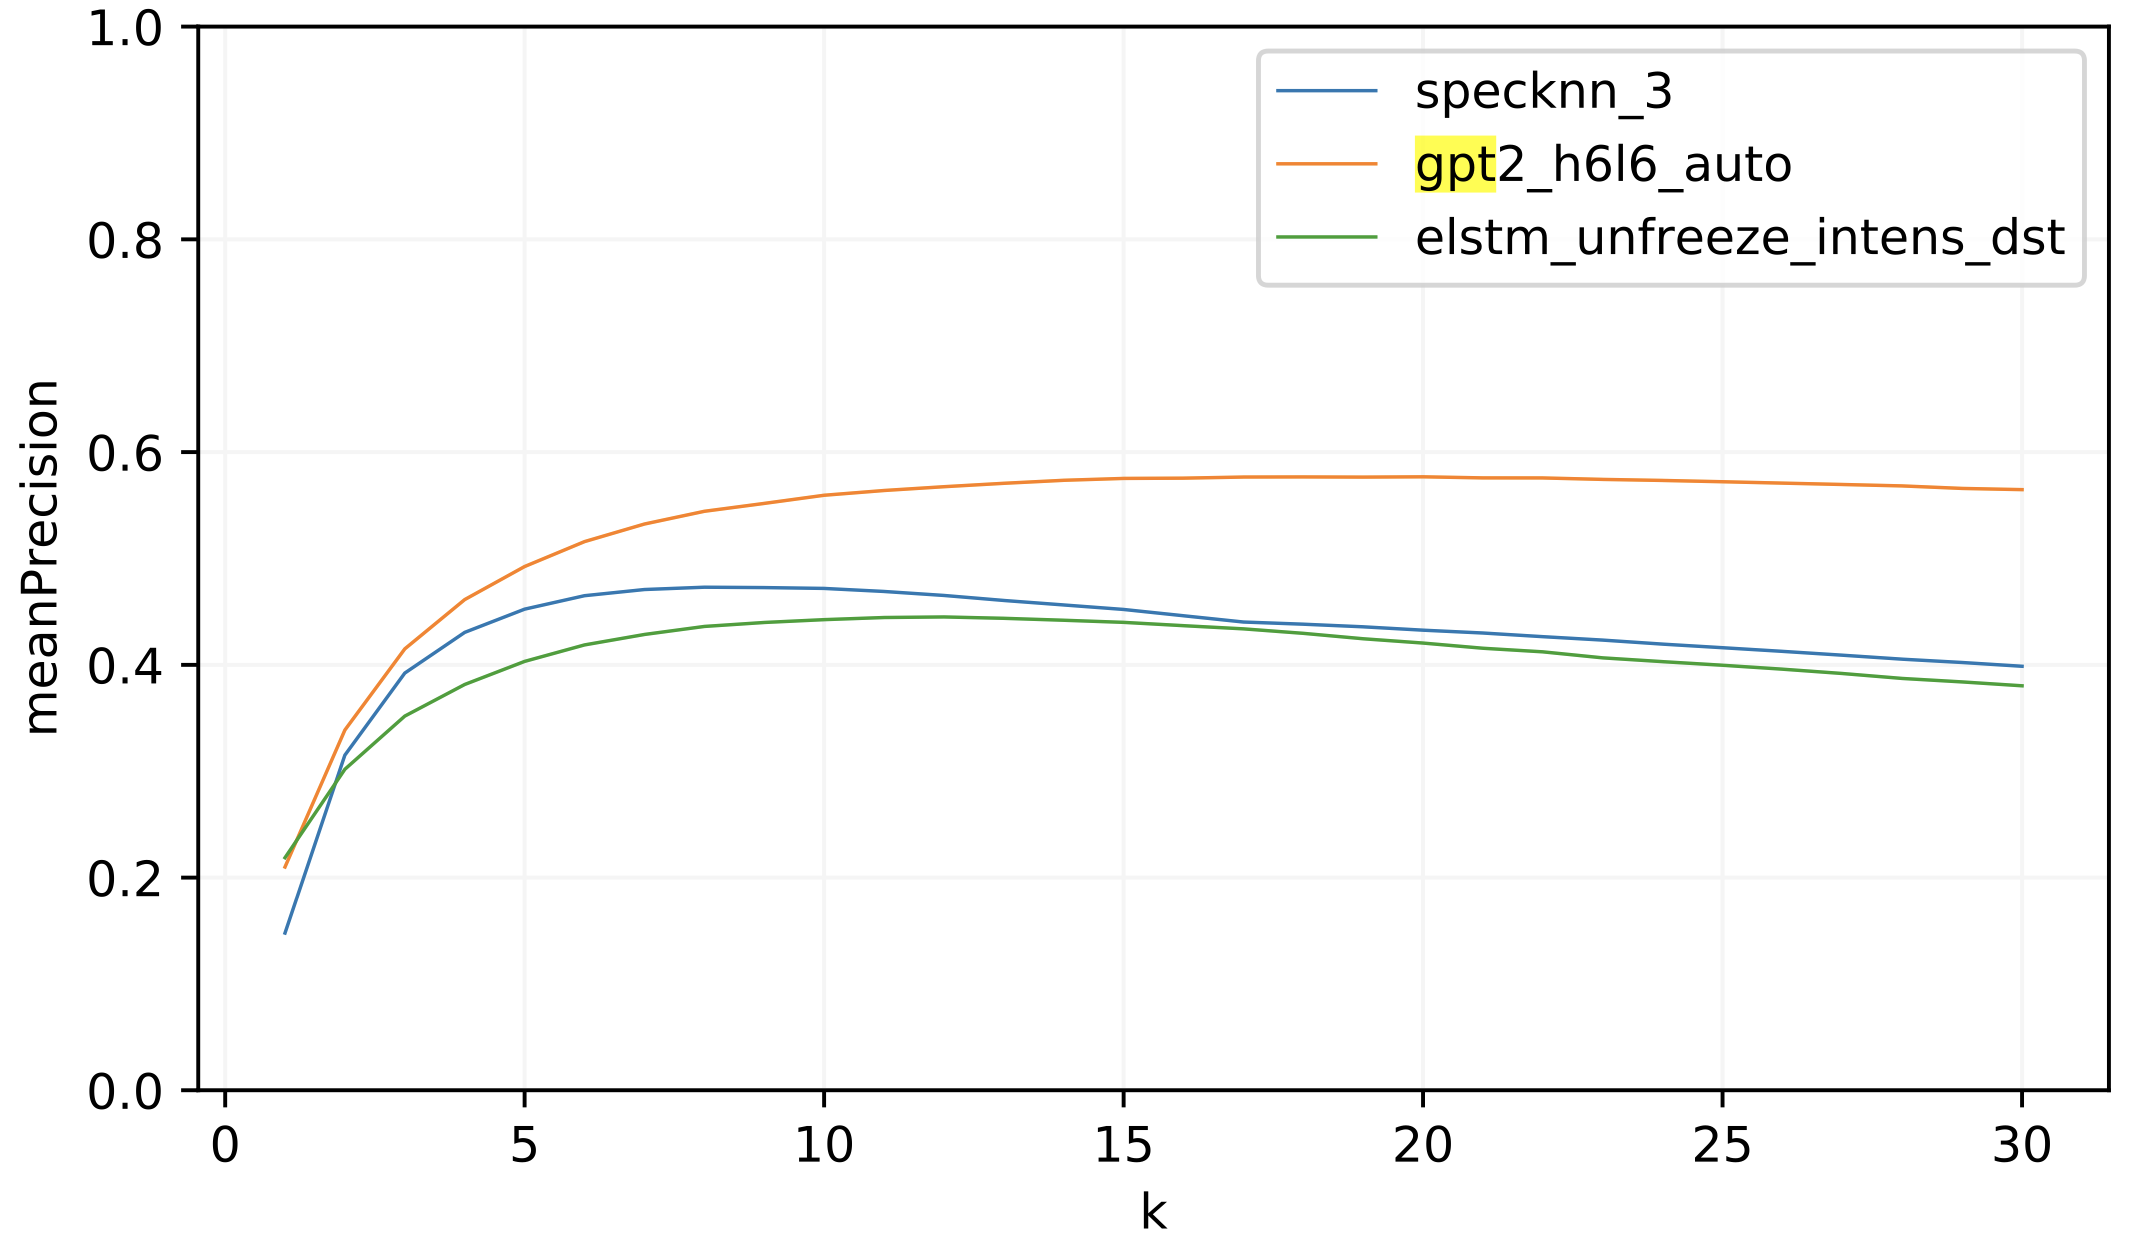
\includegraphics[width=.667\hsize]{result-missing}
\end{center}
\caption{Přesnost vybraných modelů pro predikci chybějících špiček v~prvním scénáři v~závislosti na rostoucím~$k$
(počet vstupních špiček pro model)
}
\label{f:result-missing}
\end{figure}

\begin{figure}
\begin{center}
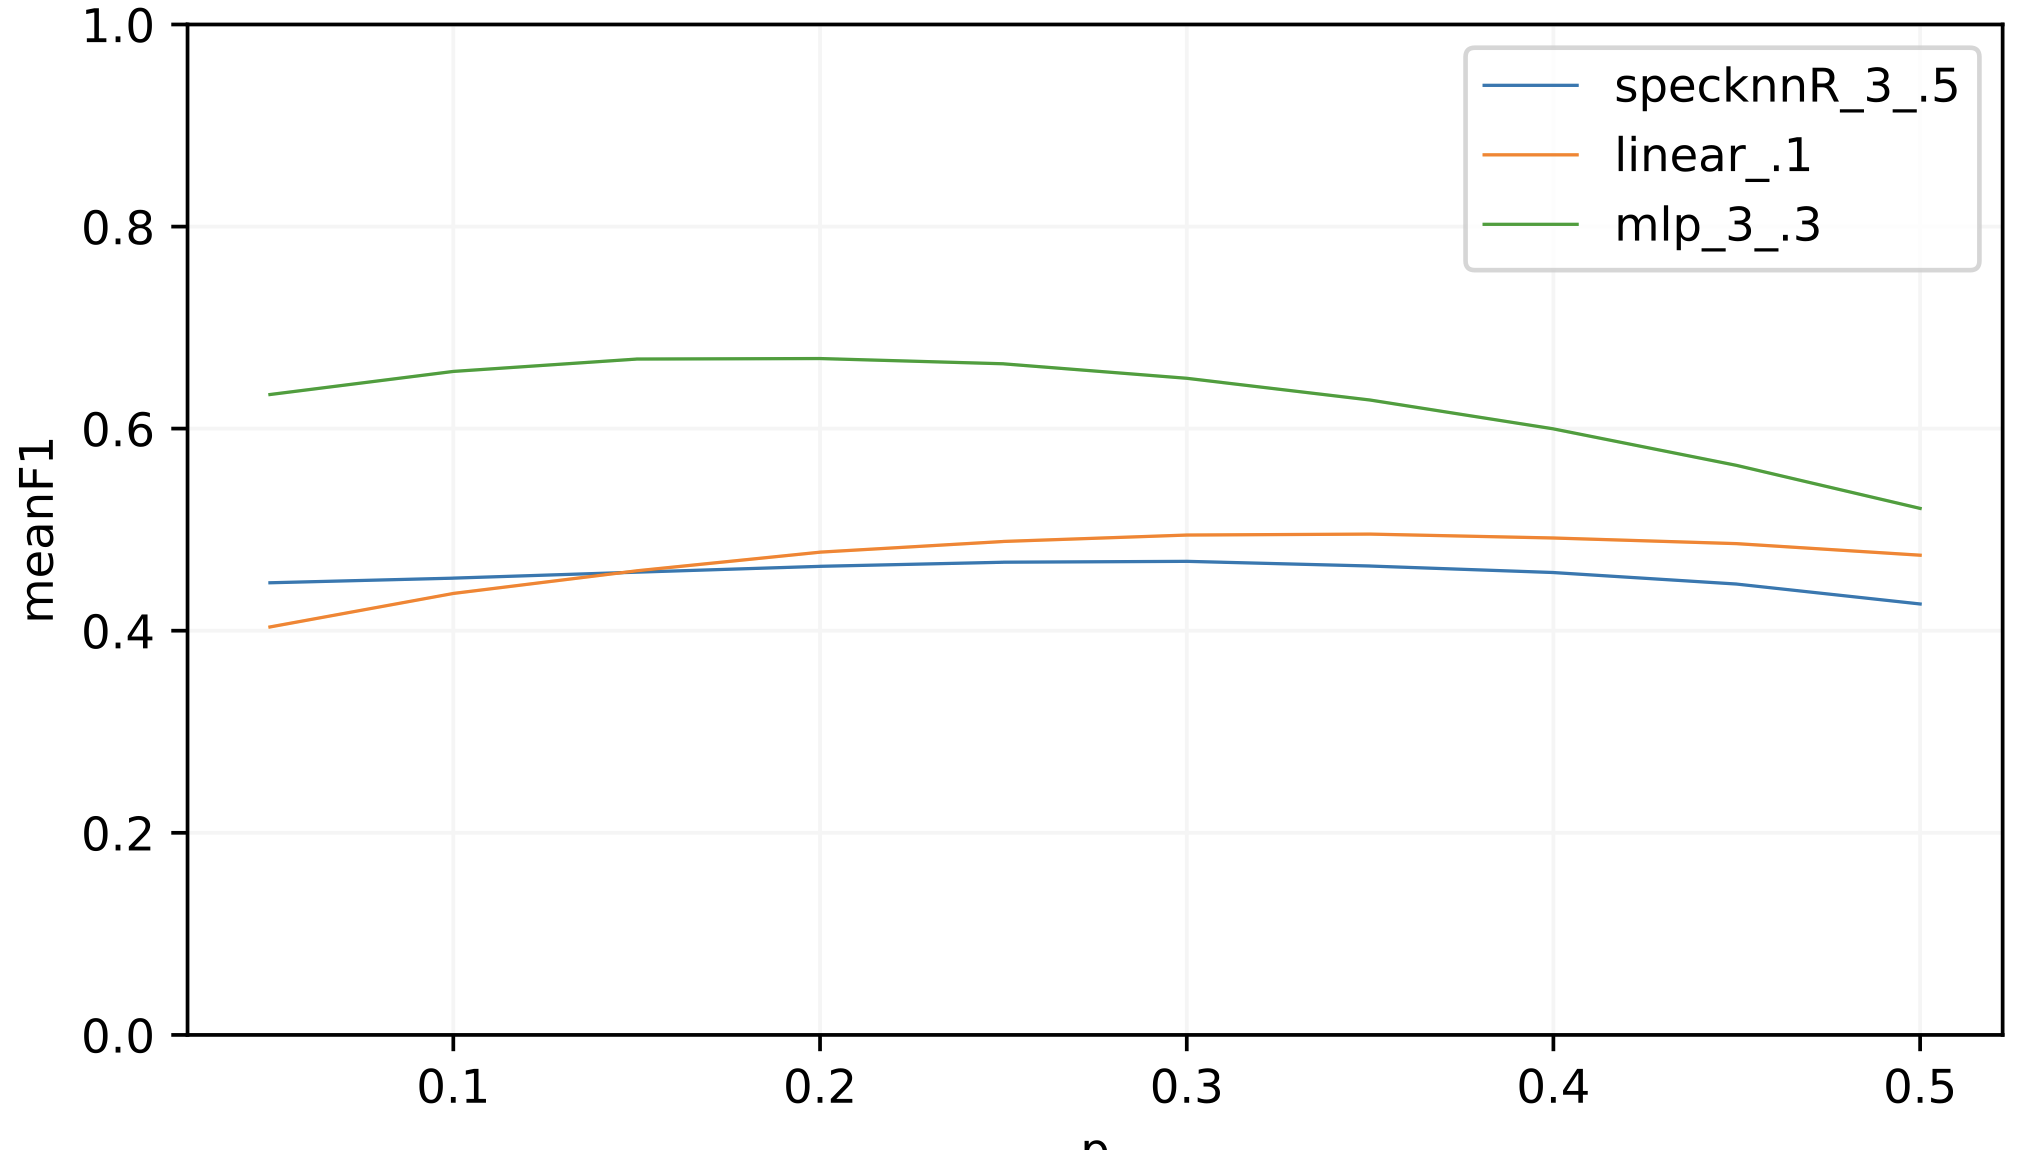
\includegraphics[width=.667\hsize]{result-wrong}
\end{center}
\caption{Přesnost vybraných modelů pro predikci chybějících špiček ve druhém scénáři v~závislosti na rostoucí
pravděpodobnosti chybějící špičky}
\label{f:result-wrong}
\end{figure}

Vytvořené modely byly dále experimentálně nasazeny jako součást komplexního workflow
v~prostředí služby UMSA (\url{http://umsa.cerit-sc.cz/}),
jehož design jsme navrhli společně s~kolegy z~centra Recetox.
Predikce chybějících špiček je nasazena do jinak konvenčního postupu zpracování 
dat z~hmotnostního spektrometru poté, co proběhne odstranění šumu a dekonvoluce signálu.
Doplněné špičky jsou heuristicky rozšířeny z~celočíselného rozsahu
(v~tom pracuje celý model, protože mnohdy historické databáze neobsahují dostatečně
zastoupená data s~vysokým rozlišením) na více možností s~vysokým rozlišením.
Takto získané špičky jsou doplněny zpět jako dodatečný vstup úplně prvního kroku
zpracování dat -- detekce špiček v~nezpracovaném signálu programem apLCMS~\cite{aplcms}
ve formě ,,nápovědy`` míst, v~nichž jsou špičky pravděpodobné (standardně je tato informace
získávána z~historických dat naměřených na konkrétním přístroji).
V~době podání této zprávy jsou k~dispozici první předběžné výsledky, které jsou na jednu stranu
slibné -- ukazuje se, že predikce v~jistých případech vylepšuje citlivost identifikace sloučenin,
ale současně narážíme na prozatím ne zcela do detailů pochopená specifika u nás získaných experimentálních
dat, která zcela neodpovídají dostupným databázím, a~tedy i trpí účinnost našich modelů.
Řešení tohoto problému bude předmětem dalšího výzkumu.




% transformery pro de-novo identifikaci, prototyp funguje, Adam bude mít diplomku


Trénování modelu predikce špiček, konkrétně model GPT-2 aplikovaný na veřejně dostupnou databázi MoNA,
jsme vyhodnotili jako vhodnou reprezentativní realistickou aplikaci pro benchmarkování výpočetních zdrojů
s~akcelerátory. 
Celý benchmark je k~dispozici ve zdrojovém kódu v~repozitáři~\url{https://github.com/RECETOX/raims/}, jeho
základní struktura byla popsána výše.

Výsledky běhu benchmarku na GPU clusterech Metacentra a CERIT-SC
(\emph{adan}, \emph{fer}, \emph{fau}, \emph{galdor}, \emph{glados} a \emph{zia})
jsou k~dispozici jako data projektu \emph{raims} ve službě Weights~\&~Biases:
\url{https://wandb.ai/ljocha/raims/}.
Díky zapouzdření v~kontejneru lze benchmarky kdykoli opakovat ve zcela identickém (s~výjimkou ovladače NVidia)
softwarovém prostředí, a tedy získat velmi dobře srovnatelné výsledky měření.
Obecně jsou výsledky ve velmi dobré shodě s~teoretickým očekáváním, což ukazuje na dobrou stabilitu
výpočetního prostředí, a celkovou zralost celého softwarového prostředí
(ovladače NVidia, knihovny CUDA, Torch, PyTorch i PytorchLightning).
Zásadním limitujícím faktorem se ukazuje velikost paměti GPU. 
Kombinace větších modelů s~větší velikostí dávky už se nepodařilo na akcelerátorech
s~menší pamětí vůbec spustit (výpočet prokazatelně končí chybovou hláškou o nepovedené alokaci paměti GPU).

V~následujícím seznamu uvádíme vybrané pozorované charakteristiky chování benchmarku se stručnými komentáři.
Je ilustrující grafy z~W\&B uvádíme pro lepší čitelnost v~příloze této zprávy.

\begin{itemize}
\item \emph{Základní srovnání výkonu GPU.} Provedeno na nejmenší konfiguraci
výpočtu (6 hlav, 6 vrstev, embedding 300, velikost dávky 64),
obr.~\ref{f:all_6_6_300_1_64_32}. 
Typy GPU jsou uspořádány v~očekávaném pořadí
T4 (adan), GeForce RTX 2080 (glados), Quadro RTX 5000 (fau), RTX A4000 (fer), A40
(galdor), A100 (zia).
Nejvýkonnější A100 (zia) předstihuje nejslabší T4 (adan) téměř čtyřnásobně.  
V~největší konfiguraci výpočtu, kterou se ještě podařilo spustit na všech typech GPU (12 hlav, 12 vrstev, embedding 300, dávka 64) je pořadí stejné, rozdíly ve výkonu jsou výraznější (obr.~\ref{f:all_12_12_300_1_64_32})

\item \emph{Spotřeba energie.} Na stejné nejmenší konfiguraci výpočtu pořadí a poměr absolutní spotřeby vesměs
odpovídá dosaženému výkonu (obr.~\ref{f:power_all_6_6_300_1_64_32}), anomálií je A100, jejíž spotřeba je výrazně nižší.

\item \emph{Vliv přesnosti výpočtu.} Použitá přesnost výpočtu (smíšená 16/32 bitů vs.\ plných 32 bitů na float)
nemá pozorovatelný vliv na přesnost modelu (obr.\ref{f:val_6_6_300_1_64_both}).
S~výjimkou nejsilnější A100, které jsou ale starší generace než A40, jsou výpočty ve smíšené přesnosti o 10--20~\% rychlejší.
Spotřeba energie je u RTX 2080, RTX 5000, A40 a A100 při použití smíšené přesnosti cca.\ o 15~\% nižší, u ostatních nemá
přesnost na spotřebu vliv.
To je opět zajímavý výsledek v~případě~A100, kde smíšená přesnost přináší energetickou úsporu aniž by ale současně
výpočet urychlila.

\item \emph{Vliv velikosti modelu.}
Velikost modelu má přímý vliv na rychlost výpočtu dle očekávání. Ukazujeme na A40, obr.~\ref{f:galdor_any_1_128_16}
s~dostatečnou pamětí pro všechny výpočty v~rozsahu počtu trénovaných parametrů 1.2--13.3 milionu.
Alokaci paměti ukazuje obr.~\ref{f:mem_galdor_any_1_128_16}, spotřebu energie obr.~\ref{f:power_galdor_any_1_128_16}.
Obojí je dle očekávání úměrné velikosti modelu, ale s~relativně malým faktorem -- více než $10\times$ větší model je pouze
$3.6\times$ pomalejší, spotřebuje o 25~\% více energie, a k~jeho běhu je třeba $4\times$ více paměti.

\item \emph{Škálování na více GPU.}
Výpočty obecně dobře škálují při spuštění na více GPU, a to už od nejmenšího modelu s~malou dávkou (obr.~\ref{f:galdor_6_6_120_any_64_both}) se zrychlením $2.15\times$ na 4 GPU
po největší model s~dvojnásobnou dávkou (obr.~\ref{f:galdor_12_12_300_any_128_both}), kde dosahujeme zrychlení $3.2\times$ na 4 GPU.
Na 8 GPU se prozatím podařilo realizovat pouze menší výpočty, při nichž přidání dalších GPU výpočet ještě zrychlí,
ale už ne významně (obr.~\ref{f:fer_6_6_120_any_64_both}).
\end{itemize}

Uvedená interpretace výsledků benchmarku zdaleka není vyčerpávající.
Kompletní datová sada je čtenáři k~dispozici na výše uvedené adrese včetně
přímo použitelných vizualizačních nástrojů pro další analýzy.


Druhá část výsledků projektu (která de-facto přesahuje rámec původního plánu) 
je implementovaný model de-novo identifikace slučenin ve fázi raného prototypu.
Kompletní zdrojový kód je k~dispozici v~\url{https://github.com/hejjack/gc-ms_bart/}.
Trénování modelu (300 mil.\ parametrů) i na relativně malé datové sadě (4.6 milionu spekter) bylo relativně náročné,
trvalo cca.\ dva dny s~využitím čtyř GPU A100.
Model dosahuje velmi dobrých výsledků na své testovací sadě generovaných spekter.
Dosavadní výsledky jsou nadějné, ale ještě ne zcela přesvědčivé na vzorcích reálných dat -- části 
databáze NIST, která nebyla použita k~trénování modelu. 
Obr.~\ref{f:bart-result} ukazuje dosavadní výsledky.
Model prokazatelně generuje podobné vzorce, ale pro přesnou identifikaci výsledky ještě 
nejsou dostatečné. 
V~další práci se zaměříme na zpřesnění vstupů i na trénování na obsáhlejší, tedy i reprezentativnější
datové sadě.

\begin{figure}
\begin{center}
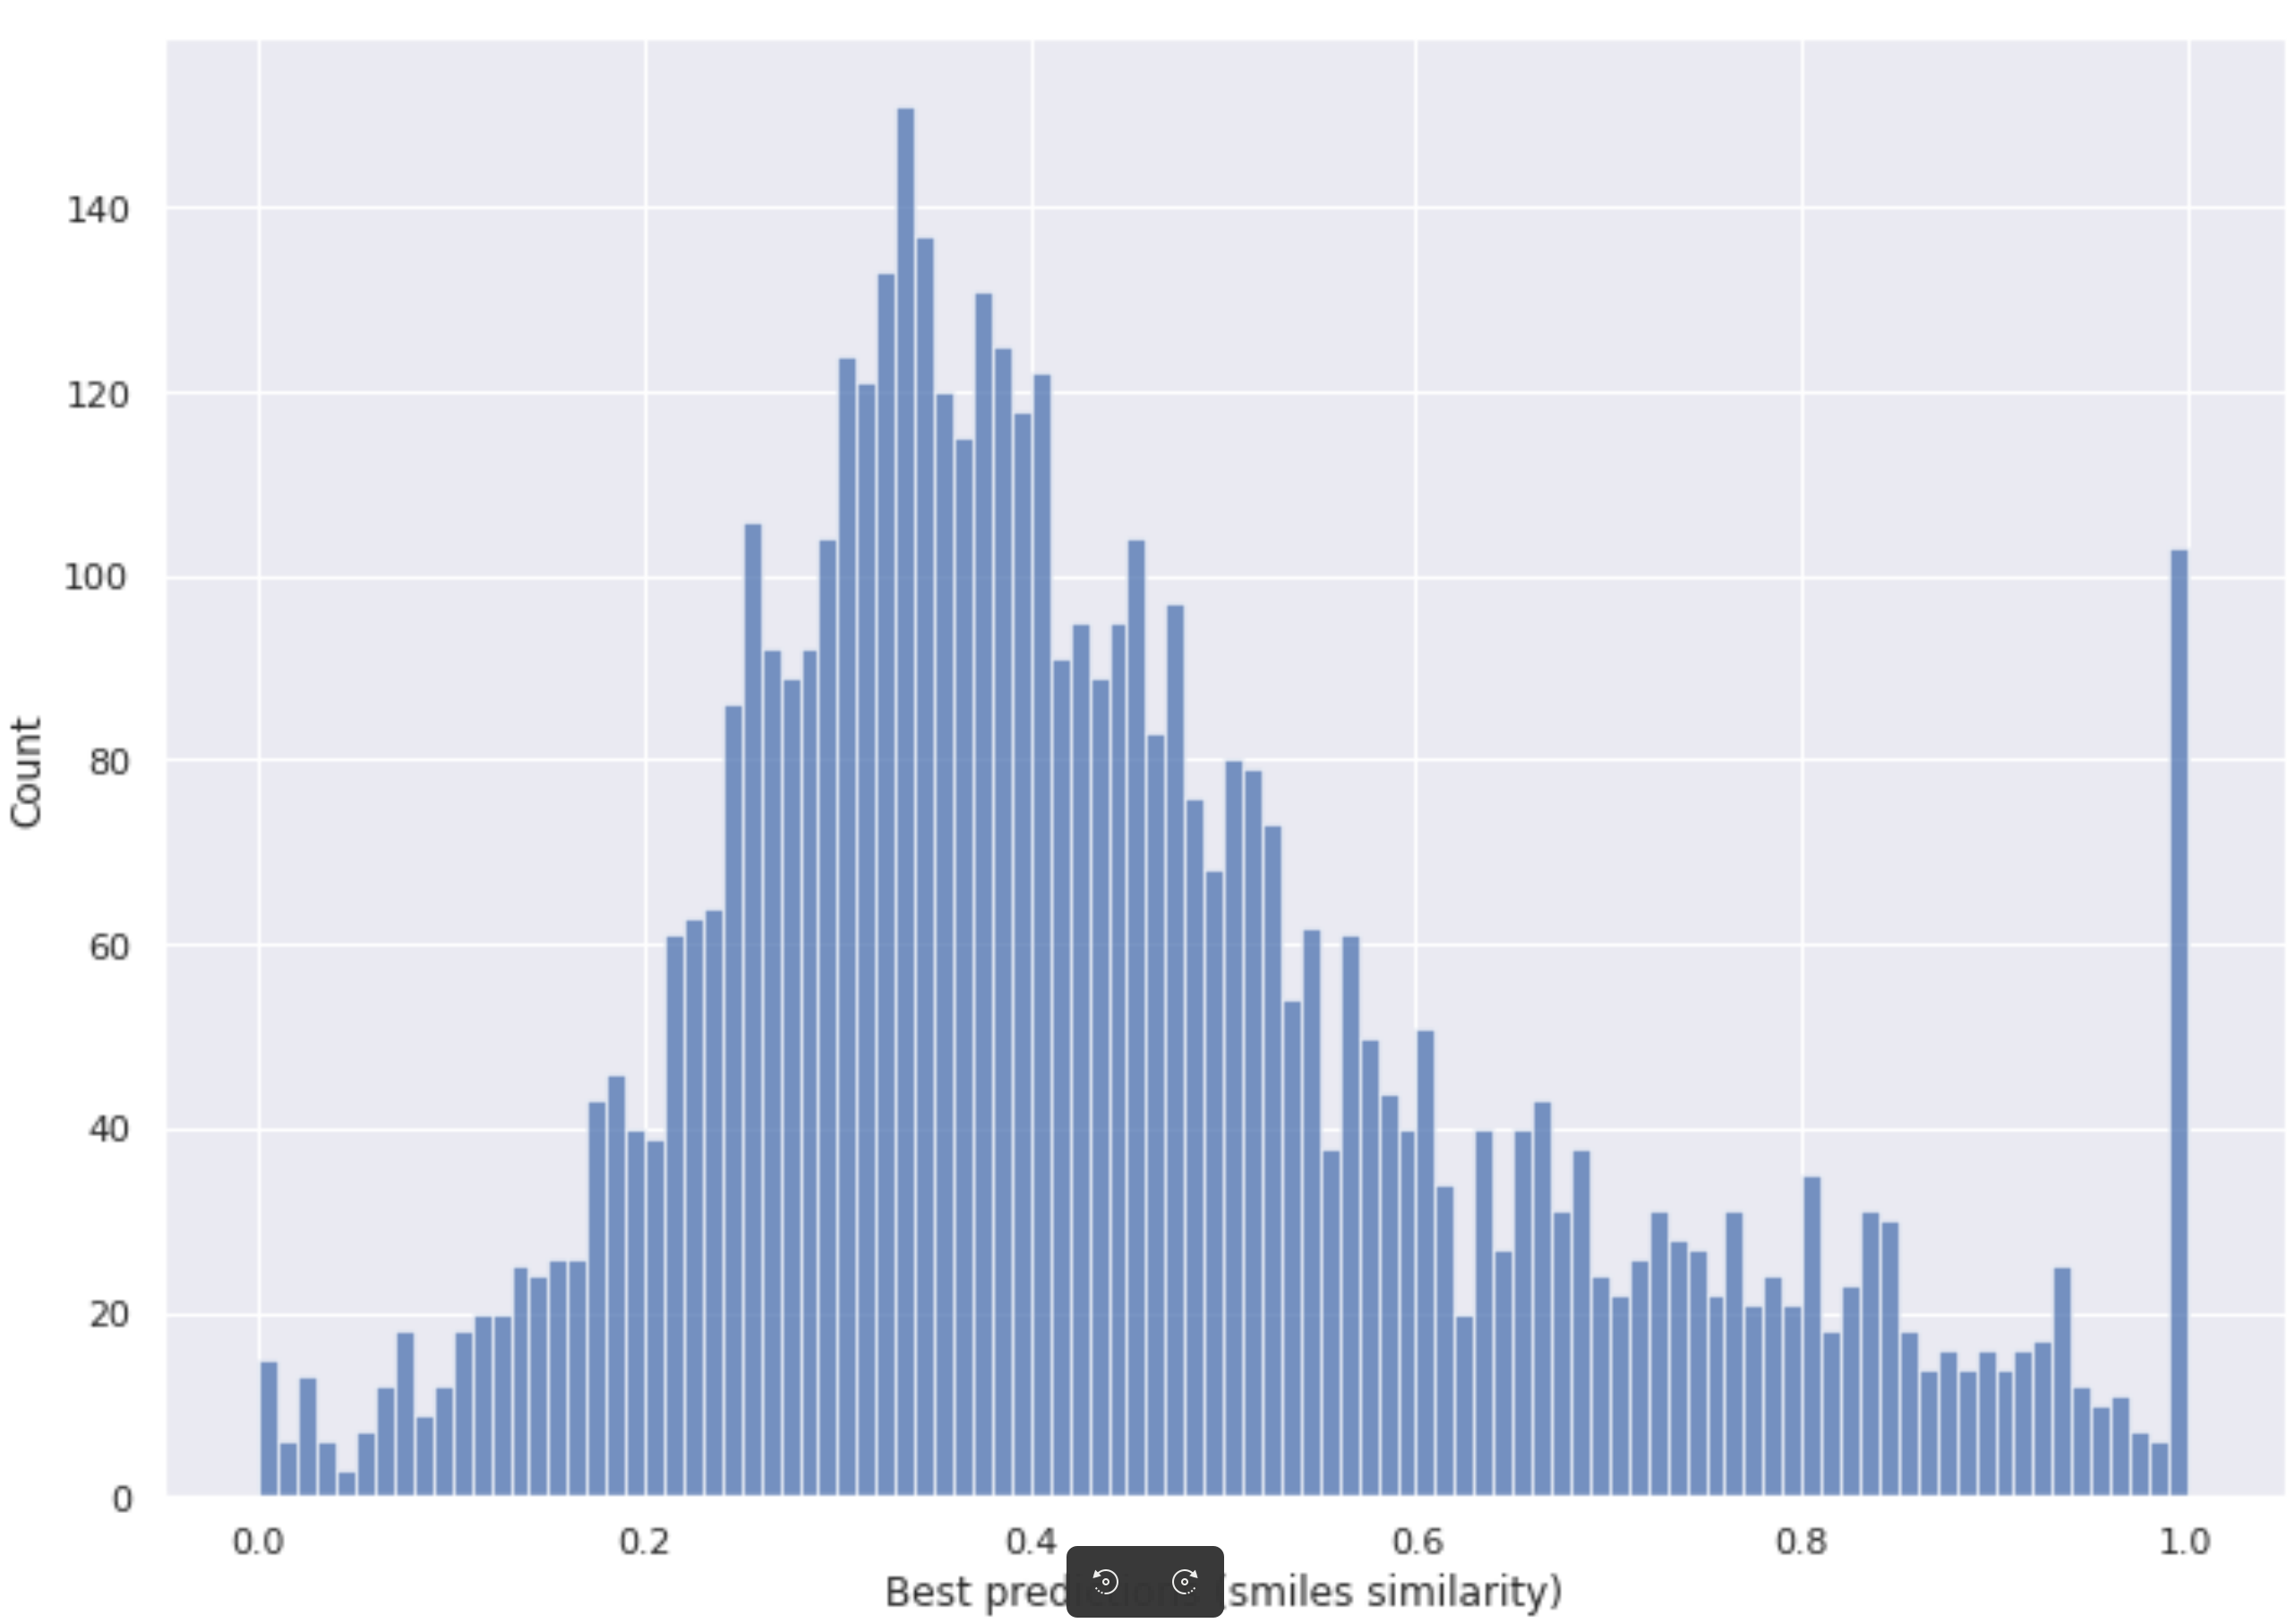
\includegraphics[width=.8\hsize]{results3_nist_on_nist}
\caption{Histogram podobnosti výstupu de-novo modelu s~referenční molekulou spočtené na fingerprintu ECFP.
Hodnoty kolem 0.5 znamenají již podobné molekuly, hodnoty nad 0.7 velmi podobné}
\label{f:bart-result}
\end{center}
\end{figure}

% Vlastní softwarový produkt (prototyp)
%• Benchmark + testovací sada
%• Dokumentace k software včetně shrnutí získaných zkušeností a doporučení pro HW/SW
%prostředí
%• Článek shrnující přínos specifického použití metod strojového učení pro aplikační oblast,
%připravený k odeslání do časopisu nebo na odbornou konferenci.
%• Certifikáty ze školení


% implementace chybějících peaků, experimentálně nasazena do Galaxy UMSA

% kód použitelný jako benchmark (github raims)


% prezentace na Metasemináři, Sitole, e-INFRA

Výsledky projektu byly prezentovány ve vystoupeních na seminářích:
\begin{enumerate}
\item Michal Starý, \emph{Prediction of missing peaks in mass spectra}, seminář laboratoře Sitola, 2.2.2022
\item Aleš Křenek, \emph{Neuronové sítě v~našich aplikacích (ty potvory vám vlezou všude)}, seminář Metacentra, Kraskov, 1.11.2022
\item Aleš Křenek, \emph{Deep learning a vrabec v~hrsti}, setkání pracovních skupin e-INFRA CZ, Ostrava, 8.11.2022
\item Adam Hájek, \emph{Experience with large-scale NLP-inspired neural networks applied in another domain}, seminář laboratoře Sitola, 16.11.2022
\end{enumerate}

Výsledkem projektu je i bakalářská práce Michala Starého, oceněná cenou děkana FI MU za vynikající závěrečnou práci.



\section{Zdůvodnění změn}

% JN hodil ručník

% proto prodloužení

% na školení jsme se vykašlali

% Adam misto Martina, kus za kus

Projekt byl významně ovlivněn dlouhodobou pracovní neschopností původního hlavního řešitele
Jiřího Novotného
a následným rozvázáním pracovního poměru z~jeho strany.
Vedení projektu proto převzal Aleš Křenek, původně pouze v~roli projektem nefinancovaného
konzultanta.
Řešení projektu (zejména vývoj benchmarku) bylo z~těchto důvodu významně zdrženo
a po dohodě s~vedením FR~CESNETu byl projekt při zachování původního rozpočtu prodloužen.
Dopad na dosažené výsledky díky tomu ale není významný.

Plánovaný softwarový prototyp, benchmark byly vyvinuty. Výsledky benchmarku jsou prezentovány
v~této zprávě, software a připravená referenční datová sada jsou použitelné pro další podobné testy.

Dosažené výsledky v~metodách doplňování chybějících špiček by dostačovaly na přípravu průměrné publikace,
jejich hlavním omezením je skutečnost, že jejich účinnost lze průkazně předvést pouze na uměle připravených
testovacích datech (byť vycházejících z~databází skutečných dat).
Proto jsme se po konzultaci s~kolegy ze spolupracujícího centra Recetox rozhodli provést ještě dodatečné
experimenty, které přenesou výsledky na reálná experimentální data.
Očekávaná publikace bude připravena až s~těmito výsledky.

Původní návrh projektu také předpokládal, že hlavní řešitel absolvuje certifikovaná školení.
S~jeho odchodem tato aktivita pozbyla smysl. Podobně zapojení studenti absolvovali ekvivalentní kursy
jako součást jejich zahraničních studijních pobytů.
Nevyužité prostředky z~této kapitoly rozpočtu vracíme.

Minoritní změnou je také zapojení Adama Hájka místo původně plánovaného Martina Kurečky.
Oba jsou pregraduální studenti, členové širšího týmu, který se zaměřuje na aplikace 
technik strojového učení v~přírodních vědách.
Pouze jejich specifické zaměření se od doby podání projektu vyvíjelo tak, že
zapojení Adama Hájka v~tomto projektu bylo přímočařejší.


\section{Přínosy projektu a hodnocení}

% po útěku JN jsme to stejně zvládli

% navaznost na H2020 EOSC Synergy

V~projektu dokončené implementace modelů pro predikci chybějících špiček v~hmotnostním spektru
a prototyp modelu pro de-novo identifikaci sloučenin jsou plně funkční, mohou být dále použity
a představují výrazný posun v~oblasti, které dovolí spolupracujícímu centru Recetox dosáhnout
na další výzkumné výsledky ve své oblasti.
Modely jsou integrovány do experimentálního workflow ve službě UMSA (jedna z~tematických služeb
projektu H2020 EOSC-Synergy).
Současně know-how získané při řešení projektu nám dovoluje v~této oblasti dále 
spolupracovat a řešit navazující problémy řešit daleko efektivněji.

Implementace také byly použity jako realistická aplikace pro benchmark GPU akcelerátorů 
a mohou být použity opakovaně pro další GPU i 
a výhledově i dalších typy akcelerátorů podporovaných frameworkem Torch.
Výsledky benchmarků přesvědčivě ukazují, že toto výpočetní prostředí je vyzrálé a stabilní
a že tento typ výpočtů v~něm dobře škáluje.
Protože benchmark je velmi dobře konfigurovatelný v~řadě parametrů, které 
ovlivňují velikost trénovaného modelu, je možné ho bezprostředně použít
i pro orientační odhad náročnosti i velmi odlišných aplikací, jeho použitelnost
tedy přesahuje původní rámec.

Přes komplikace popsané v~předchozí části se tedy cílů projektu podařilo dosáhnout
a považujeme jej za celkově úspěšný.

\section{Tisková zpráva}

V~období 7/2021--10/2022 byl realizován projekt ,,Analýza dat z hmotnostní spektrometrie za použití strojového učení``
vedený řešitelem na Ústavu výpočetní techniky MU ve spolupráci s~centrem Recetox PřF MU.
Výsledkem projektu jsou inovativní modely využívající technik strojového učení,
které výrazně vylepšují možnosti analýzy dat z~hmotnostního spektrometru.
Modely lze zároveň opakovaně využít i jako realistický benchamark výpočetních zdrojů Metacentra vybavených
akcelerátory.



\bibliographystyle{plain}
\bibliography{report}

\twocolumn
\appendix
\section{Grafy průběhu benchmarku na GPU clusterech Metacentra}

\def\graph#1#2{
\begin{figure}[h]
\begin{center}
\includegraphics[width=.95\hsize]{wandb/#1}
\caption{#2}
\label{f:#1}
\end{center}
\end{figure}
}

\graph{all_6_6_300_1_64_32}{Rychlost výpočtu v~nejmenší konfiguraci na všech clusterech}

\graph{all_12_12_300_1_64_32}{Rychlost výpočtu v~největší konfiguraci spustitelné na všech clusterech}

\graph{power_all_6_6_300_1_64_32}{Spotřeba energie v~nejmenší konfiguraci na všech clusterech}

\graph{val_6_6_300_1_64_both}{Průběh dosažené přesnosti modelu při plné a smíšené přesnosti}

\graph{galdor_any_1_128_16}{Vliv velikosti výpočtu na rychlost}

\graph{power_galdor_any_1_128_16}{Vliv velikosti výpočtu na spotřebu}

\graph{mem_galdor_any_1_128_16}{Vliv velikosti výpočtu na alokovanou paměť}

\graph{galdor_6_6_120_any_64_both}{Škálování na více GPU na malém modelu}
\graph{galdor_12_12_300_any_128_both}{Škálování na více GPU na velkém modelu}
\graph{fer_6_6_120_any_64_both}{Škálování na malém modelu až do 8 GPU}



\end{document}
